% log p(n) and log HR(n) at n=10,20,50,100, and the gap between them.
% Natural logs, recomputed from p(10)=42, p(20)=627, p(50)=204226, p(100)=190569292.
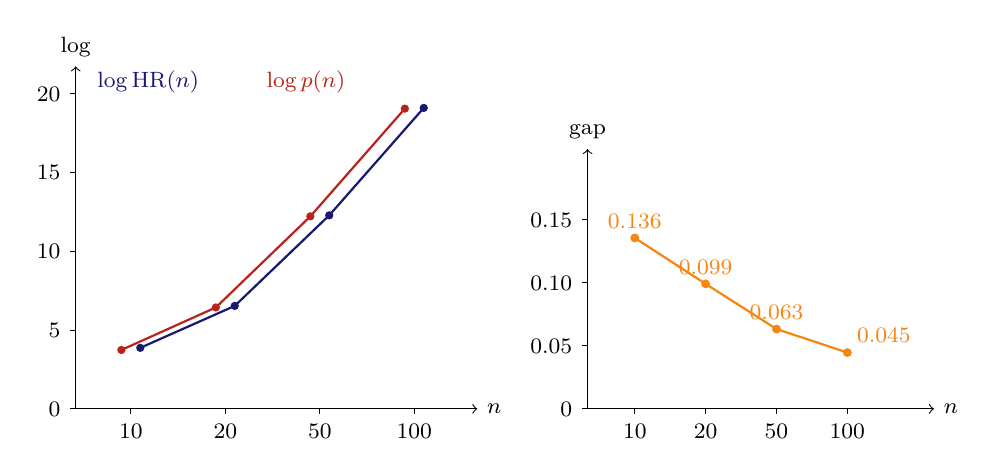
\begin{tikzpicture}[every node/.style={font=\footnotesize}]
  % Left: the two logarithms. Scale: 1 unit of log = 0.2 cm.
  \draw[->,black] (0,0)--(5.1,0) node[right] {$n$};
  \draw[->,black] (0,0)--(0,4.35) node[above] {$\log$};
  \foreach \v/\y in {0/0,5/1,10/2,15/3,20/4}{
    \draw (0,\y)--(-0.07,\y) node[left] {$\v$};
  }
  \foreach \n/\x in {10/0.7,20/1.9,50/3.1,100/4.3}{
    \draw (\x,0)--(\x,-0.07) node[below] {$\n$};
  }
  \draw[MidnightBlue,thick] (0.82,0.775)--(2.02,1.308)--(3.22,2.458)--(4.42,3.822);
  \draw[BrickRed,thick] (0.58,0.748)--(1.78,1.288)--(2.98,2.445)--(4.18,3.813);
  \fill[MidnightBlue] (0.82,0.775) circle (1.5pt);
  \fill[MidnightBlue] (2.02,1.308) circle (1.5pt);
  \fill[MidnightBlue] (3.22,2.458) circle (1.5pt);
  \fill[MidnightBlue] (4.42,3.822) circle (1.5pt);
  \fill[BrickRed] (0.58,0.748) circle (1.5pt);
  \fill[BrickRed] (1.78,1.288) circle (1.5pt);
  \fill[BrickRed] (2.98,2.445) circle (1.5pt);
  \fill[BrickRed] (4.18,3.813) circle (1.5pt);
  \node[MidnightBlue,anchor=west] at (0.15,4.15) {$\log\mathrm{HR}(n)$};
  \node[BrickRed,anchor=west] at (2.3,4.15) {$\log p(n)$};
  % Right: the gap log HR(n)-log p(n). Scale: 1 unit of gap = 16 cm.
  \begin{scope}[xshift=6.5cm]
    \draw[->,black] (0,0)--(4.4,0) node[right] {$n$};
    \draw[->,black] (0,0)--(0,3.3) node[above] {gap};
    \foreach \g/\y in {0/0,0.05/0.8,0.10/1.6,0.15/2.4}{
      \draw (0,\y)--(-0.07,\y) node[left] {$\g$};
    }
    \foreach \n/\x in {10/0.6,20/1.5,50/2.4,100/3.3}{
      \draw (\x,0)--(\x,-0.07) node[below] {$\n$};
    }
    \draw[BurntOrange,thick] (0.6,2.171)--(1.5,1.587)--(2.4,1.014)--(3.3,0.715);
    \fill[BurntOrange] (0.6,2.171) circle (1.6pt);
    \fill[BurntOrange] (1.5,1.587) circle (1.6pt);
    \fill[BurntOrange] (2.4,1.014) circle (1.6pt);
    \fill[BurntOrange] (3.3,0.715) circle (1.6pt);
    \node[BurntOrange,above] at (0.6,2.171) {$0.136$};
    \node[BurntOrange,above] at (1.5,1.587) {$0.099$};
    \node[BurntOrange,above] at (2.4,1.014) {$0.063$};
    \node[BurntOrange,above right] at (3.3,0.715) {$0.045$};
  \end{scope}
\end{tikzpicture}
